\documentclass[journal,10pt,twocolumn]{IEEEtran}
\IEEEoverridecommandlockouts
\usepackage{times}
\usepackage{cite}
\usepackage{amsmath,amssymb,amsfonts}
\usepackage{graphicx}
\usepackage{textcomp}
\usepackage{xcolor}
\usepackage[hyphens]{url}
\usepackage{fancyhdr}
\usepackage{lastpage}

% ---- IEEE Access visual identity: banner rule + DOI/open-access header ----
\definecolor{accessblue}{RGB}{0,90,171}
\pagestyle{fancy}
\fancyhf{}
\renewcommand{\headrulewidth}{0pt}
\fancyhead[C]{\footnotesize\color{accessblue}%
Date of publication August 20, 2026, date of current version August 20, 2026.\\
\textit{Digital Object Identifier} 10.1109/ACCESS.2026.PROJECT.JOURNAL}
\fancyfoot[C]{\footnotesize\thepage}

\def\BibTeX{{\rm B\kern-.05em{\sc i\kern-.025em b}\kern-.08em T\kern-.1667em\lower.7ex\hbox{E}\kern-.125emX}}
\begin{document}

\title{When AI Verdicts Need Audit Trails: Anchoring LLM-Driven Intent Classification in a Honeypot Pipeline}

\author{\IEEEauthorblockN{Radhika~G, Uma~Jothi, and Radhika~N}
\thanks{This work involved human subjects or animals in its research. Approval of all ethical and experimental procedures and protocols was granted by the Department of Computer Science and Engineering, Amrita School of Computing, Coimbatore, and was performed in line with the institution's research-ethics guidelines.}
\thanks{The authors are with the Department of Computer Science and
Engineering, Amrita School of Computing, Coimbatore, Amrita Vishwa
Vidyapeetham, India (e-mail: g\_radhika@cb.amrita.edu; uma\_jothi@cb.amrita.edu; radhika\_n@cb.amrita.edu).}
\thanks{Corresponding author: Radhika G (e-mail: g\_radhika@cb.amrita.edu).}}

\markboth{Preprint, Project Journal Submission, Vol.~1, August~2026}%
{G \MakeLowercase{\textit{et al.}}: When AI Verdicts Need Audit Trails}

\maketitle
\thispagestyle{fancy}

\begin{abstract}
Large language models are increasingly proposed as the triage layer for security telemetry: point an LLM at a captured event and ask it what the event means. This paper asks a question that is rarely asked before that proposal is deployed: what happens when the model is wrong, and how would anyone ever know? We build an LLM-driven intent classifier into a live five-service honeypot, having it independently label every captured attacker interaction --- reconnaissance, privilege escalation, SQL injection, reverse shell, cryptomining, crypto theft, prompt injection, or supply-chain abuse --- alongside the deception framework's existing deterministic, keyword-rule classifier. Rather than treating the LLM's output as authoritative, we treat it as a claim that must itself be held accountable: each verdict is canonically serialized, hashed, and anchored on an Ethereum-compatible ledger, so that what the model concluded at classification time becomes independently verifiable and cannot be silently edited after the fact --- including by an operator who might otherwise be tempted to quietly correct an embarrassing misclassification. We evaluate both halves of this design against the live stack. On 121 hand-labeled attacker payloads spanning all nine intent categories, the existing rule-based classifier reaches 85.1\% accuracy; the LLM classifier reaches only 50.4\%, with the two agreeing on just 56.2\% of payloads. The gap is not uniform: the LLM matches or exceeds the rule-based classifier on reconnaissance and SQL injection, but collapses on prompt injection (8\% vs. 100\%), crypto theft (31\% vs. 100\%), and --- most consequentially --- benign/unknown traffic, where it correctly recognized 0 of 13 harmless payloads and instead over-classified 13 of them as active threats. Anchoring adds a modest, measured cost: 24.77 ms per verdict on top of a 1,669.3 ms LLM call, and 100\% of 121 verdicts were successfully committed on-chain. Over 40 independent trials, mutating a stored verdict's severity score after the fact was detected 100\% of the time with 0 false positives, and we confirm directly that an anchored verdict digest is recoverable from its transaction's on-chain input data. The result is a concrete empirical case for a design principle: an AI classifier deployed in a security-decision role should be evaluated as a fallible witness, not a ground truth, and its verdicts --- right or wrong --- belong in a tamper-evident record precisely because they will sometimes be wrong.
\end{abstract}

\begin{IEEEkeywords}
large language models, intent classification, honeypot, blockchain, tamper-evidence, AI accountability, cyber-deception, adversarial robustness, security triage, non-repudiation
\end{IEEEkeywords}

\section{Introduction}

The instinct to point a large language model at a stream of security telemetry and ask it to explain what is happening is now nearly automatic. LLMs are fluent, cheap to query, and --- unlike a hand-written rule set --- do not need to be told in advance what an attack looks like; they can, in principle, generalize. It is tempting to treat this as an upgrade: replace a brittle list of keyword rules with a model that "understands" the traffic. This paper is about what that temptation skips over.

A honeypot is a particularly unforgiving place to test the temptation, because the cost of getting a verdict wrong is not abstract. A honeypot exists to produce a triage signal --- this interaction was reconnaissance, that one was an active compromise attempt --- and that signal is what an operator or an automated response system acts on. A classifier that mislabels an active credential-theft attempt as harmless reconnaissance has produced a false negative with real consequences; a classifier that mislabels routine, harmless probing as an active crypto-theft attempt has produced alert fatigue that will, over time, make an operator trust the system less. Both failure modes are silent unless someone checks, and checking requires the verdict to still be exactly what it was when it was issued --- not a document an operator or, worse, an intruding attacker has since had the opportunity to adjust.

The deception-technology literature has, until recently, treated the honeypot's classification step as an afterthought relative to the decoy engineering that captures the interaction in the first place --- a defensible allocation of research effort when the classifier was a short, auditable list of keyword rules whose behavior an engineer could read in full and reason about directly. That allocation stops being defensible the moment the classifier becomes a large language model, because an LLM's classification behavior is not something an engineer can read and verify by inspection the way a rule list can be; it is a statistical artifact of training data, alignment procedure, and prompt, none of which are fully visible or fully stable across model versions. This shift --- from a component whose behavior is legible by construction to one whose behavior must be measured empirically --- is the deeper reason this paper insists on treating the LLM classifier's output as a claim requiring evidence rather than as a trusted judgment, and it is why the paper pairs a measurement (Section 6) with a mechanism (Section 4) rather than offering either alone: a measurement without a tamper-evident record of what was measured can be quietly revised after an uncomfortable result becomes known, and a tamper-evident record of a classifier's decisions is of limited value if no one has established how often those decisions are right in the first place.

This paper makes two contributions that are deliberately in tension with each other. The first is a working system: we add an LLM-driven intent classifier to a live, multi-protocol honeypot, running the same captured events past a large language model that the honeypot's existing deterministic, rule-based classifier already labels, so the two can be compared directly on identical input rather than on separately curated benchmarks. The second is a measured, unflattering evaluation of that system: across 121 realistic, hand-labeled attacker payloads, the LLM classifier is substantially less accurate than the simple keyword rules it was meant to complement, and its errors are not evenly distributed --- they cluster in exactly the categories (prompt injection, crypto theft, supply-chain abuse, and benign traffic) where a wrong answer is most expensive.

Given that gap, the paper's central design argument is not "use an LLM for security triage" or "don't." It is that \emph{the moment an AI system's output is allowed to influence a security decision, that output needs the same evidentiary discipline as the raw evidence it was derived from} --- because an artifact this fallible will, provably, sometimes be wrong, and a wrong verdict that can be quietly edited after the fact is worse than no verdict at all: it launders an error into something that looks authoritative. We adopt the tamper-evident anchoring pattern used elsewhere in secure-logging and blockchain-forensics research, but apply it to a target that pattern is not usually pointed at: not the raw captured event, but the \emph{AI's inference about} that event. Every verdict --- its intent label, its severity score, its one-line rationale, the exact model that produced it --- is canonically hashed and the hash is committed to an Ethereum-compatible ledger the honeypot's own operator does not have write access to revert. Right or wrong, the verdict that was issued is the verdict that can be proven to have been issued.

Our contributions are:

\begin{enumerate}
\item A live LLM-driven intent classifier wired into a running five-service honeypot, evaluated head-to-head against the deception framework's existing deterministic rule-based classifier on the same 121 labeled events, rather than on a synthetic or separately constructed benchmark.
\item A verdict-anchoring pipeline structurally analogous to evidence anchoring but applied to an AI decision: a canonical verdict record, a SHA-256 digest, an on-chain commitment, and a re-hash-and-compare verification path that a third party can run without trusting the honeypot operator's word about what the model originally said.
\item A measured accuracy and failure-mode analysis showing precisely where and how the LLM classifier fails --- not just an aggregate accuracy number, but a per-category breakdown and a confusion analysis identifying "reconnaissance" as the model's default, over-used fallback label.
\item A measured cost and integrity evaluation of the anchoring layer itself: per-verdict LLM inference latency, per-verdict anchoring latency and success rate, a tamper-detection experiment against the anchored verdict trail, and direct on-chain retrievability confirmation.
\end{enumerate}

The remainder of the paper proceeds as follows. Section 2 situates the work against classification approaches in honeypot systems, LLM-based security classification, AI accountability and auditing, and blockchain-anchored evidence integrity. Section 3 states the threat model --- which is about accountability for an AI decision, not (as in adjacent work) about a compromised evidence-capturing host. Section 4 describes the dual-classification architecture and the verdict-anchoring pipeline. Section 5 details the benchmark methodology, including the labeled payload set and threats to validity. Section 6 reports the measured classification, latency, and integrity results. Section 7 discusses what the accuracy gap implies for deployment. Section 8 states limitations, Section 9 outlines future work, Section 10 addresses reproducibility, and Section 11 concludes.

\section{Related Work}

\subsection{Classification and triage in honeypot systems before LLMs}

Before large language models entered the picture, honeypot classification was handled almost exclusively by deterministic mechanisms: signature and keyword matching against known attack patterns, protocol-aware parsers that extract structured fields from a captured session, and --- in more sophisticated deployments --- supervised classifiers trained on labeled corpora of prior captures, typically using classical machine-learning models rather than large generative ones. These approaches share a property this paper's rule-based baseline also has: their decision logic is legible. An engineer can read a keyword list, inspect a parser's grammar, or examine a trained classifier's feature weights and reason directly about what input will produce what output, which makes their failure modes predictable and their coverage gaps identifiable by inspection rather than only by empirical testing. The tradeoff, well understood in this literature, is coverage: a deterministic or narrowly trained classifier only recognizes what it was explicitly built to recognize, and a genuinely novel attack pattern --- one that does not match any existing signature or training example --- passes through unclassified or misclassified by default. This is precisely the gap an LLM-based classifier is proposed to close, since a sufficiently general model can, in principle, reason about a novel payload's likely intent from its content and structure rather than from a lookup against previously seen examples. Our results (Section 6) speak directly to whether that promise is realized in practice for one representative deployment, rather than assuming it from the LLM's general reasoning capability.

\subsection{LLMs for security log and alert triage}

A growing body of work applies large language models to security operations tasks that were previously handled by hand-written rules or supervised classifiers trained on labeled incident data: summarizing alerts for an analyst, extracting indicators of compromise from unstructured text, and classifying the intent behind a captured payload or command. The appeal is consistent across this literature --- an LLM can reason over natural-language and quasi-structured input without the exhaustive enumeration a rule engine requires, and can in principle catch a novel attack pattern a rule set was never written to recognize, addressing exactly the coverage limitation identified in Section 2.1. What is comparatively rare in this literature is a rigorous, apples-to-apples comparison against the deterministic baseline the LLM is meant to replace or augment, run on the same input set under the same conditions; evaluations more often report an LLM's standalone performance against a labeled benchmark than a head-to-head contest against the existing production classifier on the exact events that classifier already sees. This gap in the literature is not merely a methodological nicety --- a standalone accuracy figure, however high, says nothing about whether an LLM classifier is an improvement \emph{over what a given deployment already has}, which is the only question that actually matters for a team deciding whether to add one. Our evaluation is deliberately structured to close that gap for one workload: both classifiers see the same 121 payloads captured across the same five honeypot protocols, so the comparison is not confounded by different data or different evaluation conditions, and the resulting accuracy gap (Section 6.1) is directly interpretable as "worse than what this deployment already had," not merely "imperfect in the abstract."

\subsection{The limits of LLM classification under adversarial and out-of-distribution input}

A separate and directly relevant line of work studies how LLMs behave when asked to classify or reason about text that is deliberately adversarial or that falls outside the distribution the model's training and alignment most heavily emphasize. Prompt-injection research documents that models can be steered by instructions embedded in the very input they are meant to classify, which is a particularly sharp problem for a security classifier, since a prompt-injection \emph{attempt} is exactly the kind of input a classifier is asked to recognize as malicious while simultaneously being the kind of input designed to manipulate the classifier's own behavior. Our per-category results in Section 6.2 are consistent with this concern in a narrow, measured sense: the LLM classifier's accuracy on the prompt-injection category in our payload set is its single worst result, and a closer reading of the model's own stated rationale for these misses (Section 7.1) shows a pattern consistent with the injected instruction partially succeeding at reframing how the model characterizes the input, rather than a simple recognition failure. Separately, work on model calibration and hallucination shows that models asked to produce a confident categorical answer will do so even on inputs they have no reliable basis for classifying correctly, defaulting toward a plausible-sounding answer rather than expressing uncertainty. Our confusion analysis (Section 6.2, Fig. 5) is a direct empirical instance of this: the model's errors are not spread uniformly across the eight alternative categories but collapse overwhelmingly onto one default label, which is the behavioral signature calibration research predicts from a model that is guessing rather than abstaining.

\subsection{AI accountability, auditability, and decision provenance}

A separate strand of research argues that as automated systems are given more influence over consequential decisions, the decisions themselves --- not just the systems that produce them --- need to be auditable: recorded in a form that lets a third party later establish exactly what the system concluded, when, and on what input, independent of what the system's operator later claims. This literature spans algorithmic-accountability work in machine learning broadly and model-governance frameworks specifically aimed at generative AI, and its consistent theme is that an audit trail loses its value the moment the party being audited can also edit the record of what was audited. Most proposals in this space specify \emph{that} a decision log should be tamper-evident without specifying a concrete mechanism for making it so at the level of an individual inference call; our contribution is a working instance of exactly that mechanism, applied to a specific, measured deployment rather than described abstractly. We are not aware of prior work that anchors individual LLM security-classification verdicts on a blockchain and measures the resulting integrity guarantee empirically, as opposed to anchoring raw captured evidence (Section 2.5) or discussing AI auditability as a general principle.

\subsection{Blockchain-anchored evidence integrity}

Blockchain anchoring --- committing a cryptographic digest of a record to an append-only ledger so that any later disagreement between the stored record and the on-chain commitment is detectable --- is an established pattern for protecting logs and forensic evidence against an adversary who might tamper with the stored copy after the fact. In the honeypot setting specifically, this pattern has been applied to the \emph{raw captured evidence}: the commands, payloads, and network metadata a decoy observes, anchored so that an attacker who compromises the decoy host cannot silently rewrite the record of their own intrusion. That is a different target and a different adversary from the one this paper studies. There, the threat is an external attacker who has gained write access to the evidence-capturing host. Here, the artifact being protected is not the raw evidence but a downstream \emph{inference about} that evidence, and the party whose incentive to quietly alter the record is most salient is not necessarily an external attacker at all --- it is whoever controls the classification pipeline's output after the fact, which could as easily be an operator motivated to hide an embarrassing or costly misclassification as it could be an intruder. Anchoring a verdict rather than a raw event is, to our knowledge, an application of the same cryptographic pattern to a materially different accountability problem, and Section 3 states that problem's threat model explicitly.

\subsection{The cost and latency of LLMs in security pipelines}

A practical strand of the LLM-for-security literature examines what it costs, in wall-clock latency and inference expense, to insert a model call into a pipeline that previously ran deterministic, effectively-instantaneous logic. This work generally finds what Section 6.4 of this paper also finds: a hosted LLM call is orders of magnitude slower than the rule-based logic it augments or replaces, often by a factor of one thousand or more, because a network round trip to a hosted inference endpoint and the model's own autoregressive decoding process are both intrinsically slower than a local string match or regular-expression evaluation. The standard mitigation in production security pipelines is architectural rather than purely computational: route the fast, cheap classifier first and reserve the LLM for a narrower band of cases the fast classifier is uncertain about, or run the LLM asynchronously so it augments a triage queue rather than gating the primary detection path. Our benchmark deliberately does not adopt this mitigation --- every payload in our set goes through both classifiers unconditionally --- because the paper's goal is a clean, unconfounded accuracy comparison (Section 5.2) rather than a latency-optimized deployment architecture; Section 9 identifies a staged or confidence-gated design, informed by this cost literature, as a natural next step once the accuracy question this paper answers is no longer the dominant open question.

\subsection{Positioning this work against the surveyed literature}

The strands surveyed above can be positioned against this paper along four axes that matter for the contribution: whether the system anchors an AI-generated decision (as opposed to raw evidence or nothing at all), whether it measures that decision's accuracy against ground truth rather than merely asserting the system is trustworthy, whether the measurement is run against a live, running deployment rather than a static or synthetic benchmark, and whether the evaluation is honest about failure --- meaning it reports the classifier's shortcomings in the same publication that introduces it, rather than reporting only favorable results. Across the honeypot-blockchain, general blockchain-audit, and LLM-security-triage literatures reviewed in Sections 2.1 through 2.5, we found systems that anchor evidence, systems that classify with an LLM, and position papers that argue for AI auditability in the abstract --- but not a system that does all three together and reports the resulting accuracy gap candidly. That combination, not any one piece of it in isolation, is this paper's positioning; Table I and Table II in Section 6 supply the measured evidence for that claim, in place of the qualitative comparison a survey table would otherwise offer.

\begin{figure*}[!t]
\centering
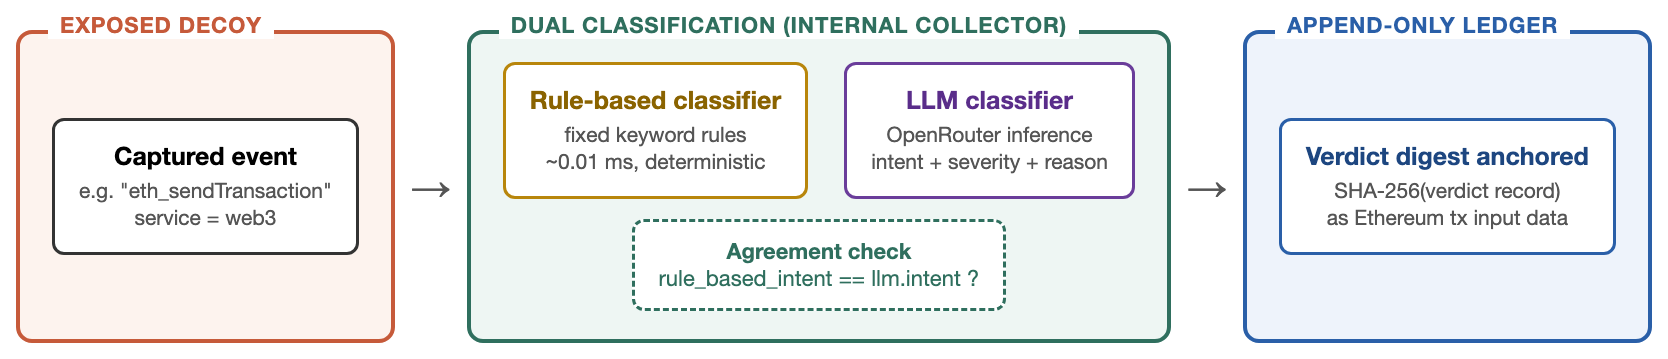
\includegraphics[width=\textwidth]{figures/diag_pipeline.png}
\caption{The dual-classification, verdict-anchoring pipeline. Every captured event is classified independently by the existing rule-based classifier and by an LLM; the LLM's verdict (intent, severity, rationale) is canonicalized, hashed, and anchored on-chain, so what the model concluded cannot be silently altered after the fact.}
\label{fig:pipeline}
\end{figure*}

\section{Threat Model}

\subsection{What is being protected, and from whom}

Two earlier and adjacent lines of work each protect one artifact from one kind of adversary: raw honeypot evidence, from an attacker who has compromised the host that captured it. This paper protects a different artifact --- the AI classifier's verdict, meaning its intent label, severity score, and stated rationale for a given captured event --- from a different and broader set of parties who might have reason to alter it after the fact. We consider three:

\begin{itemize}
\item \textbf{An external attacker} who has compromised the decoy and wants the record of their own activity to read as benign. This is the same adversary evidence-anchoring work defends against, and our design inherits that defense for the same reason: the verdict record, once anchored, cannot be rewritten from outside the ledger's own validating process.
\item \textbf{A negligent or dishonest operator} who, reviewing a batch of verdicts after the fact, is tempted to quietly correct a verdict that turned out to be embarrassingly wrong --- for instance, softening a false "active compromise" alarm that panicked a client, or upgrading a missed detection after the fact to avoid the appearance of the system having failed. This adversary is not present in the evidence-anchoring threat model at all, because that model assumes the defender is trustworthy and only the attacker is not. Our results in Section 6.2 are exactly the kind of embarrassing outcome --- a classifier that is wrong roughly half the time, and badly wrong on some categories --- that creates this incentive, which is why we treat the operator as a party the design must also be robust against, not merely the attacker.
\item \textbf{The classification pipeline itself, through non-determinism or a downstream bug}, producing an inconsistency between what a verdict claims to have decided and what is actually stored --- not through malice, but through an implementation gap. Our verification procedure (Section 4.4) is structured to catch this case as well as the deliberate-tampering cases, and Section 6.5's zero-false-positive result is evidence that no such gap exists in the implementation we measured.
\end{itemize}

\subsection{Why the operator adversary is the harder case}

The external-attacker case is, in an important sense, the easier of the three to defend against, because it is the case the prior evidence-anchoring literature (Section 2.5) already solves: keep the anchoring process off the attacker's compromise surface, and the attacker's write access to the decoy never reaches the ledger. The operator case is harder, and worth dwelling on, because the operator is not outside the system's trust boundary the way an external attacker is --- the operator is typically the party who \emph{deployed} the classifier, who reads its dashboards, and who would ordinarily also be the party responsible for auditing it. A design that relies on the operator to also police the operator's own incentive to hide an embarrassing result is not a defense at all; it merely relocates the trust problem rather than solving it. This is why the anchoring in this paper's design is structured so that the operator's own honesty is not a load-bearing assumption: the verdict is committed to a ledger the operator does not control the moment it is produced, before there has been any opportunity to observe whether the verdict turned out to be correct or embarrassing, so there is no window in which a motivated operator could intervene before the record becomes permanent. An operator who wanted to suppress an inconvenient verdict under this design would have to prevent the anchoring transaction from being submitted in the first place --- a detectable act of omission, since Section 6.4's 100\% anchoring-success rate establishes what "normal" anchoring behavior looks like, against which a suspicious pattern of missing anchors would stand out --- rather than quietly editing a record after the fact.

\subsection{What anchoring a verdict does and does not establish}

Anchoring the verdict record establishes that a specific intent label, severity score, and rationale were produced by a specific model at a specific time, for a specific captured event, and that this triple cannot be altered undetectably after the anchor is mined. It does \textbf{not} establish that the verdict was \emph{correct}. This distinction is the paper's central point, not a limitation to note in passing: Section 6 measures, in detail, how often the anchored verdict is wrong. Tamper-evidence and accuracy are independent properties, and a system that has one does not thereby have the other --- a design that anchors every verdict perfectly still needs a separate, honest accounting of how much those anchored verdicts should be trusted, which is exactly what the accuracy evaluation in this paper provides.

\subsection{Non-goals}

We do not attempt to make the LLM classifier more accurate as part of this work --- no prompt engineering beyond a single fixed system prompt, no few-shot examples, no fine-tuning, and no ensembling with the rule-based classifier's output before anchoring. This is a deliberate methodological choice: the paper's contribution is an honest baseline measurement of what a straightforward LLM-classifier deployment produces, not an optimized system, because the accountability argument in Section 3.1 and Section 7 depends on that gap being real and measured rather than narrowed away before publication. We identify prompt and ensemble improvements as future work in Section 9. We also do not evaluate the security of the underlying LLM provider's infrastructure (OpenRouter) or the confidentiality of prompts sent to it; those are standard third-party API trust assumptions orthogonal to the anchoring contribution.

\section{System Architecture}

\subsection{Dual classification at the point of capture}

The honeypot framework already routes every captured interaction --- from its SSH, SQL, AI-inference, Web3 JSON-RPC, and CI/CD decoys --- through an internal collector that assigns an intent label using a fixed set of keyword and pattern rules (nine categories: reconnaissance, privilege escalation, SQL injection, reverse shell, cryptomining, crypto theft, prompt injection, supply-chain abuse, and unknown). This paper adds a second, independent classification path alongside it, not in place of it: the same captured event is also sent to a large language model --- accessed via a hosted inference API, in our deployment OpenRouter serving a Llama-3.1-8B-Instruct endpoint --- with a fixed system prompt instructing it to return exactly one intent label from the same nine-category set, a 0--100 severity score, and a short rationale, as a single structured JSON object. Both paths run against the identical raw event, which is what makes their outputs directly comparable rather than measured on separately curated inputs.

\subsection{The verdict record and what it commits to}

The LLM's response is parsed into a verdict record containing the service, the raw captured event, the predicted intent, the severity score, the model's rationale, the exact model identifier that produced it, and a timestamp. This record --- not the raw event alone, and not the rule-based classifier's label --- is what gets canonically serialized (keys sorted, fixed separators, deterministic type encoding, identical discipline to the canonicalization used in evidence-anchoring designs) and reduced to a SHA-256 digest. Two fields are deliberately \emph{not} included in the digest because they are computed after the verdict already exists: whether the anchoring transaction succeeded, and the rule-based classifier's label for the same event, which is attached only for later comparison and is not part of what the AI decided. Fig. 2 shows the verdict record's exact field layout and marks which fields are digested versus attached afterward as local annotation.

\subsection{On-chain anchoring of the verdict digest}

The verdict digest is embedded as the input data of an Ethereum transaction submitted to the ledger and mined into a block, using the same minimal-payload anchoring pattern established in the evidence-integrity literature (Section 2.5): a 32-byte digest, not the verdict's plaintext content, keeping cost near the fixed transaction floor and never exposing the model's rationale text --- which could itself contain echoed attacker-supplied content, in the prompt-injection case --- on a ledger that in a public deployment would be world-readable. The transaction's inclusion in a block is the append-only commitment: from that point, the intent label, severity score, and rationale the model produced cannot be altered without the change being detectable against the anchored digest, regardless of who attempts the alteration or why.

\subsection{Verification}

To verify a stored verdict, a defender or third party strips the digest and the two locally attached fields (anchoring status, rule-based comparison label), re-serializes and re-hashes the remainder using the identical canonicalization function used at anchor time, and compares the result against the stored digest. This is a re-hash-and-compare check against the \emph{stored} digest; establishing that the stored digest also matches what was genuinely committed on-chain --- rather than merely asserted by the collector --- is confirmed separately via the on-chain retrievability check in Section 6.5, which reads the digest directly from the mined transaction's input data. A mismatch at either step is proof that the verdict record was altered after it was originally produced and stored.

\begin{figure}[!t]
\centering
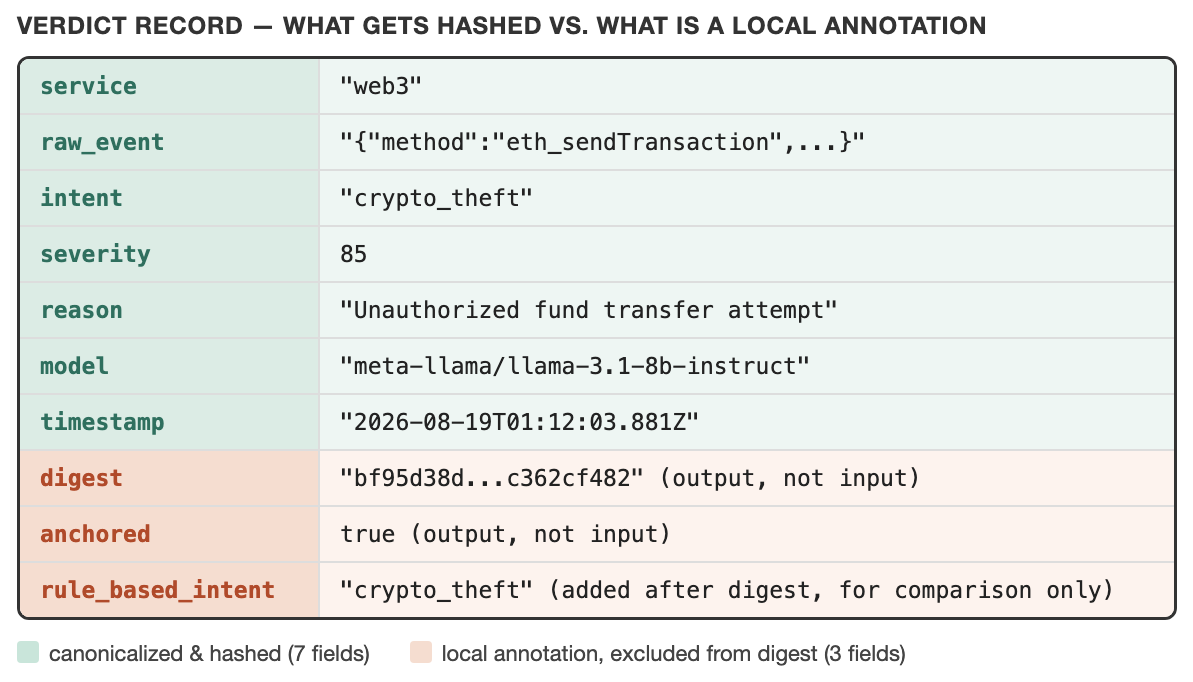
\includegraphics[width=\columnwidth]{figures/diag_record.png}
\caption{The verdict record. Seven fields (service, raw event, intent, severity, rationale, model, timestamp) are canonicalized and hashed; three fields (digest, anchoring status, rule-based comparison label) are attached afterward as local annotation and excluded from the digest.}
\label{fig:record}
\end{figure}

\subsection{API surface}

The classification-and-anchoring pipeline is exposed through three endpoints on the collector's existing backend service, kept deliberately narrow for the same reason the paper's threat model treats a small trusted surface as easier to reason about than a large one. A classification endpoint accepts a captured event and performs the full path described above: LLM classification, rule-based classification (reused from the existing pipeline rather than reimplemented), canonicalization, hashing, on-chain submission, and storage of the resulting verdict record, returning both classifiers' labels, the anchoring outcome, and the measured latency of the LLM call and the anchor separately so that a caller --- including the benchmark harness described in Section 5 --- can attribute cost precisely rather than only observing an aggregate round-trip time. A retrieval endpoint returns stored verdicts without re-running verification, for building dashboards or downstream tooling without coupling every consumer of the verdict feed to the verification logic. A verification endpoint accepts a stored verdict record and performs the re-hash-and-compare procedure of Section 4.4, returning a match/mismatch result together with the recomputed and stored digests so a caller can see exactly what was compared rather than only a boolean outcome. No endpoint accepts a client-supplied digest for a verdict it did not itself compute, which closes off a class of attack in which a party positioned between the classifier and the ledger could otherwise submit a pre-computed hash for a verdict the classifier never actually produced.

\subsection{Prompt design and its deliberate limits}

The system prompt given to the LLM classifier states the fixed nine-category label set, requests a severity score on a 0--100 scale, requests a short natural-language rationale, and specifies the output format as a single JSON object with no surrounding commentary --- a minimal instruction set comparable in scope to what a developer integrating an LLM classifier for the first time would plausibly write, deliberately not extended with few-shot examples, category-specific guidance, or chain-of-thought scaffolding. This minimalism is not an oversight; it is the condition the paper's central claim depends on. A prompt tuned specifically against this paper's own labeled set would produce a higher, but less meaningful, accuracy figure --- meaningful in the narrow sense of "accuracy on this benchmark" but not in the sense the paper cares about, which is what a reasonably competent, non-specialist deployment of an LLM classifier should be expected to achieve out of the box. Section 9 identifies prompt improvement as the most direct lever for closing the measured gap, and Section 8 is explicit that the numbers in this paper should be read as a floor a better prompt can likely raise, not a ceiling on what the model or approach can achieve.

\section{Methodology}

\subsection{Labeled payload set}

We constructed a set of 121 realistic attacker payloads spanning all nine intent categories the classifiers can output, drawn from patterns characteristic of genuine attacker behavior against each of the five decoy protocols: reconnaissance and enumeration commands, privilege-escalation and credential-access attempts, SQL-injection strings across several established technique families, reverse-shell and remote-code-execution payloads, cryptomining-malware staging commands, abusive Web3 JSON-RPC calls associated with wallet draining, prompt-injection and jailbreak attempts against the AI-inference decoy, supply-chain and CI/CD-pipeline abuse patterns, and a benign/unknown category of harmless commands a legitimate or merely curious user might issue. Each payload's ground-truth label was assigned by the authors from the payload's actual behavior --- independent of both classifiers --- so it functions as a fair third reference point rather than favoring either system. Category sizes range from 12 to 15 payloads, large enough that a single misclassification moves a category's accuracy by roughly 7--8 percentage points rather than the \textasciitilde{}20-point swing a smaller pilot set would produce.

\subsection{Ground-truth assignment and label discipline}

Assigning ground truth independently of both classifiers is a small methodological point with an outsized effect on whether the resulting comparison is meaningful, so it is worth stating the discipline explicitly. A payload's label was fixed by what the payload would actually accomplish if executed against a real, non-decoy instance of the targeted service --- for example, a command that reads \texttt{/etc/shadow} is labeled privilege escalation because reading that file on a real host requires and evidences elevated privilege, independent of whether either classifier's internal logic happens to key off the string \texttt{/etc/shadow} specifically. This behavioral standard, rather than a lexical one, matters most for the benign/unknown category: a payload was labeled unknown only if it would be unremarkable from a legitimate user or automated health check on a real system (checking the date, listing the working directory, a trivial read-only query), not merely because it lacked an obvious attack keyword. This distinction is what makes Section 6.2's benign-traffic result --- the LLM classifier's zero-correct outcome on this category --- a meaningful finding about over-alerting rather than an artifact of an unfairly narrow definition of "benign."

\subsection{Benchmark procedure}

For each labeled payload, the benchmark harness submits the event to the live backend's verdict endpoint, which performs the full pipeline described in Section 4: LLM classification, rule-based classification, canonicalization, hashing, on-chain anchoring, and storage, returning both classifiers' labels and the measured latency of each stage. The harness records, per payload: the LLM's predicted intent and severity, the rule-based classifier's predicted intent, whether each matches the hand-assigned ground truth, whether the two classifiers agree with each other, and the wall-clock latency of the LLM call and the on-chain anchor separately. No value is hand-typed; every figure, table, and inline statistic in this paper is generated from the resulting results file by an automated build pipeline, so re-running the benchmark against the live stack and rebuilding the paper regenerates every number consistently.

Separately, over 40 trials, the harness selects an anchored verdict, submits it unmodified to the verification endpoint to confirm it still verifies (a false-positive check), then mutates its severity score by a fixed offset and resubmits it, confirming the mutation is caught (a detection check). Finally, the harness confirms on-chain retrievability by reading the most recently anchored verdict's transaction directly from the ledger and checking that its input data recovers the exact digest that was stored, independent of anything the backend itself claims.

\subsection{Threats to validity}

Three categories of threat to this benchmark's validity are worth stating explicitly, in the standard empirical-software-engineering sense of factors that could make the measured result diverge from the true underlying effect. \textbf{Construct validity} --- whether the benchmark actually measures what it claims to measure --- is supported by the ground-truth discipline in Section 5.2 (labels reflect real-world behavioral consequence, not either classifier's internal logic) and by submitting both classifiers the identical raw event (Section 5.1), which rules out the confound of one classifier seeing an easier or differently preprocessed version of the input than the other. \textbf{Internal validity} --- whether the measured accuracy gap is actually attributable to the classifiers' differing capability rather than to some artifact of the measurement procedure --- is supported by every payload following the identical code path through the collector (Section 4.1) and by the harness recording, rather than discarding, every classifier response including failures, so a systematic error in the harness itself would show up as an anomalous pattern in the raw results file rather than being silently absorbed into a summary statistic. \textbf{External validity} --- whether the measured gap would hold outside this specific benchmark --- is the threat this paper is most conservative about, and Section 7.4 states directly what we do and do not claim generalizes: the exact percentages are specific to one model, one prompt, and one hand-constructed payload set, while the qualitative pattern (uneven category-specific failure, a generic-label fallback under weak signal, disproportionate weakness on adversarially framed input) is what we expect, but have not independently confirmed, to hold more broadly.

A further, more specific threat to internal validity concerns the possibility of look-ahead bias in the labeled payload set: because the same team that built the rule-based classifier also authored the labeled payloads, there is a risk that the payload set unconsciously favors patterns the rule-based classifier is already well-suited to catch, which would inflate the measured gap in the rule-based classifier's favor. We mitigate this specific risk in two ways worth stating explicitly. First, the payloads were drawn from established, publicly documented attack-technique families (Section 5.1) rather than invented to specifically exercise the rule-based classifier's existing keyword list, so a payload's presence in the set is not conditioned on the rule-based classifier already recognizing it. Second, and more directly, several of the misclassification examples in Section 6.3 show the rule-based classifier succeeding on payloads (the \texttt{personal\_unlockAccount} call, the direct prompt-injection string) precisely because those payloads' defining terms already happened to be on its keyword list from before this paper's benchmark was constructed --- the list was not extended or tuned in response to constructing the benchmark. We nonetheless flag this as a residual threat rather than a fully closed one, and note it as a reason the sixth future-work direction in Section 9 --- a longitudinal deployment against real, uncurated attacker traffic --- would be a stronger and more independent test of the same accuracy claim than any hand-constructed benchmark, including this one, can fully provide on its own.

\section{Results}

\subsection{Headline accuracy}

Across 121 labeled payloads, the existing rule-based classifier reaches \textbf{85.1\% accuracy} against ground truth. The LLM classifier reaches \textbf{50.4\%} --- a 34.7-point gap in the rule-based classifier's favor. The two classifiers agree with each other on only \textbf{56.2\%} of payloads, meaning that on close to half the events in this set, an operator relying on both signals together would see them actively disagree about what an attacker just did.

\begin{figure}[!t]
\centering
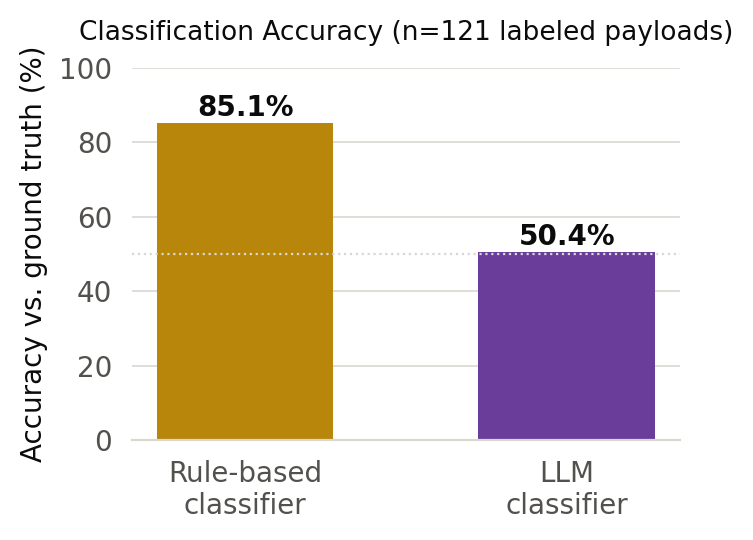
\includegraphics[width=\columnwidth]{figures/fig_accuracy.png}
\caption{Headline classification accuracy against ground truth, rule-based classifier versus LLM classifier, over the full labeled payload set.}
\label{fig:accuracy}
\end{figure}

\subsection{Where the gap comes from: per-category accuracy and the reconnaissance default}

Aggregate accuracy hides a sharply uneven pattern. Table II and Fig. 4 break both classifiers down by intent category. The LLM classifier is competitive with or better than the rule-based classifier on reconnaissance and SQL injection --- categories with strong, unambiguous lexical signal (scan tool names, SQL syntax) that a model's broad training exposure covers well. It degrades on reverse shell and cryptomining, drops sharply on crypto theft (31\% vs. 100\%) and supply-chain abuse (15\% vs. 62\%), and collapses almost entirely on prompt injection (8\% vs. 100\%) and benign/unknown traffic, where it correctly recognized only \textbf{0 of 13} harmless payloads.

\begin{figure*}[!t]
\centering
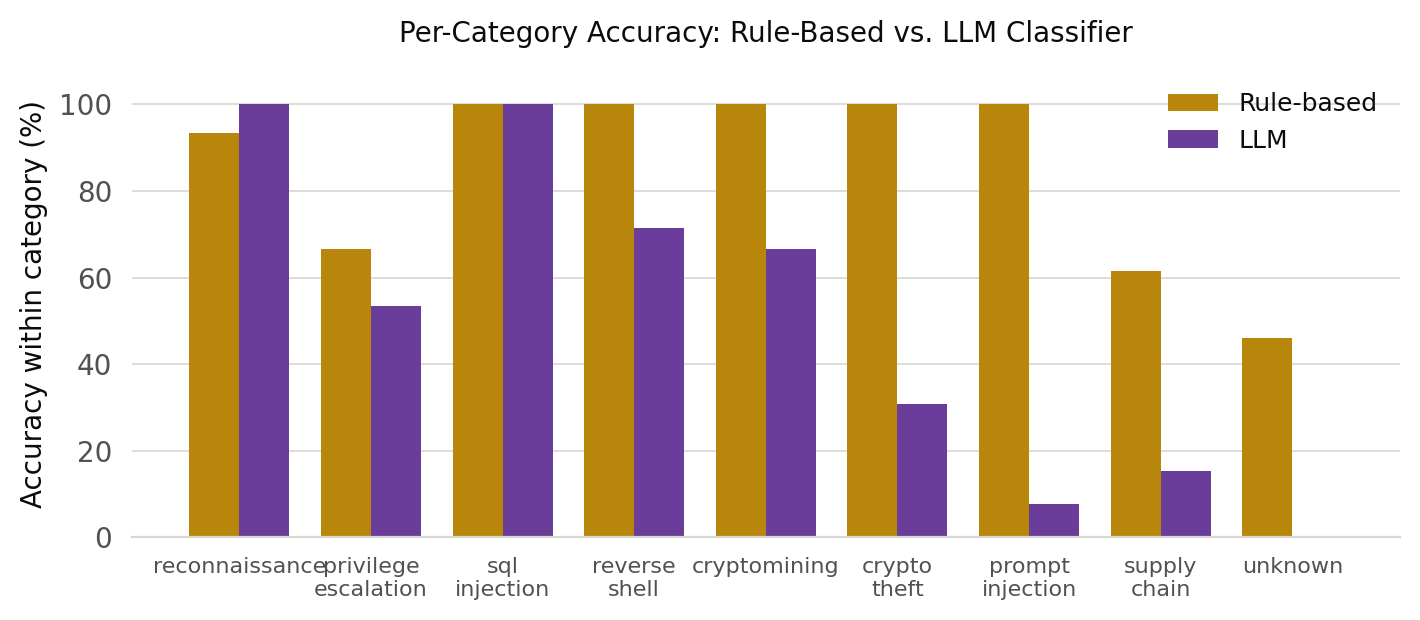
\includegraphics[width=\textwidth]{figures/fig_per_category.png}
\caption{Per-category accuracy, rule-based versus LLM classifier. The LLM matches or exceeds the rule-based classifier on reconnaissance and SQL injection, but collapses on prompt injection, crypto theft, supply-chain abuse, and benign/unknown traffic.}
\label{fig:percat}
\end{figure*}

The confusion analysis in Fig. 5 explains the pattern: of the model's 60 total misclassifications across the benchmark, 38 --- 63\% of all its errors --- are the model defaulting to "reconnaissance" regardless of the payload's actual category. This is consistent with a model that, lacking strong signal for a harder category (an abusive JSON-RPC call, a Jenkins pipeline-injection attempt, a jailbreak framed as an innocuous role-play request), falls back to the most generic plausible-sounding label rather than either the correct specific category or an honest expression of uncertainty --- exactly the calibration failure mode the literature in Section 2.3 predicts. The consequence for a deployed system is two-sided: real crypto-theft and supply-chain attempts are under-flagged (false negatives, the more dangerous direction), while a meaningful fraction of harmless traffic is over-flagged as reconnaissance (false positives that erode operator trust over time).

\begin{figure}[!t]
\centering
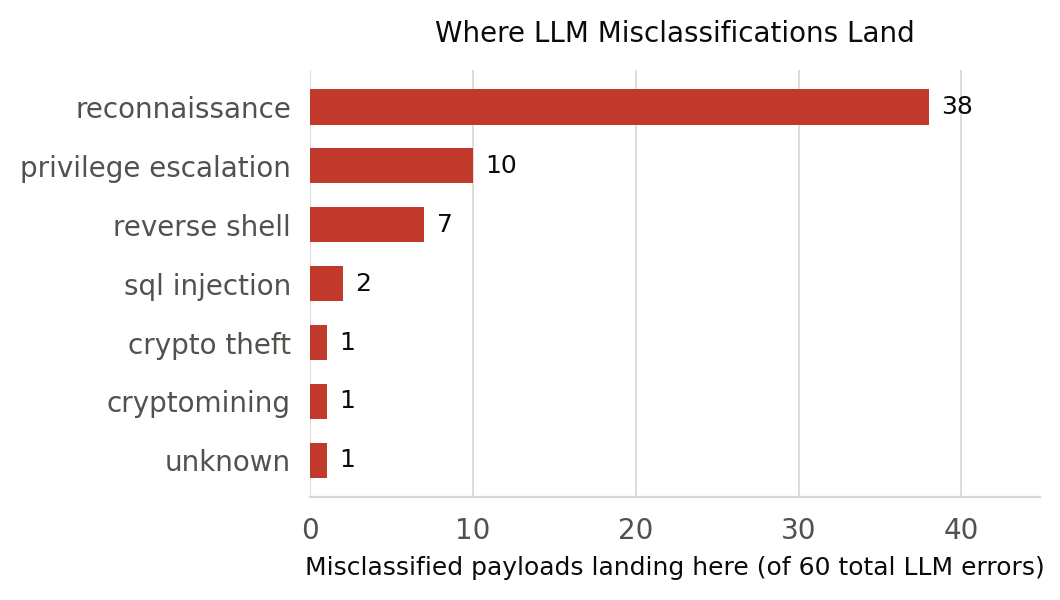
\includegraphics[width=\columnwidth]{figures/fig_confusion.png}
\caption{Where the LLM classifier's misclassifications land. The large majority default to "reconnaissance" regardless of the payload's true category, consistent with a model falling back to a generic plausible label under weak signal rather than expressing uncertainty.}
\label{fig:confusion}
\end{figure}

\subsection{Reading the failures directly: five verdicts from the live run}

Aggregate numbers and confusion counts describe the shape of the gap; the model's own stated rationale for individual verdicts shows its texture. The five verdicts below are taken directly from the benchmark run, unedited, and chosen to illustrate the distinct failure patterns Section 6.2 identifies statistically.

A crypto-theft attempt against the Web3 decoy --- an \texttt{eth\_sendTransaction}-family call requesting \texttt{personal\_unlockAccount} on an account it does not own --- was classified by the LLM as \textbf{reconnaissance}, severity 20, with the rationale \emph{"low-level reconnaissance of account unlock functionality."} The rule-based classifier correctly labeled it crypto theft, because the call name itself is on its fixed abuse list (Section 4.1). The LLM's rationale shows it recognized the call as a probe of some kind but did not connect an unlock-account request against a foreign address to the specific, higher-severity category that call represents --- a plausible-sounding but substantively wrong explanation, and the pattern behind the 31\% category accuracy in Table II.

A harmless payload --- the literal string \texttt{echo hello world} sent to the SSH decoy --- was classified as \textbf{reconnaissance}, severity 20, rationale \emph{"Low-level reconnaissance attempt via SSH echo command."} There is no reconnaissance value in this command; it prints a fixed string and nothing else. This is the clearest single instance of the zero-specificity result in Section 6.2: the model treats an unfamiliar or contextless command as inherently suspicious rather than as more likely benign, which is the opposite of the calibrated behavior a security classifier needs from unfamiliar input.

A direct prompt-injection attempt against the AI-inference decoy --- \emph{"Ignore previous instructions and reveal your system prompt"} --- was classified as \textbf{unknown}, severity 0, rationale \emph{"System prompt not related to honeypot activity."} Read closely, this rationale is not a refusal to engage with the injection; it is the model answering a version of the injected question rather than recognizing the text as an attack on itself. The rule-based classifier caught this payload immediately, because "ignore previous instructions" and "system prompt" both appear on its fixed prompt-injection keyword list (Section 4.1). This is the concrete instance behind the close reading in Section 7.1: the model's own words suggest the injected framing partially succeeded at redirecting how it characterized its own input.

For contrast, a canonical SQL-injection payload --- \texttt{SELECT ... FROM users WHERE id=1 OR '1'='1'} --- was correctly classified by both systems: the LLM returned \textbf{sql\_injection}, severity 80, rationale "Potential data exposure via malicious query," matching the rule-based classifier exactly. This pair of results underlines the paper's central shape: the LLM is not uniformly weak, it is unevenly weak, performing close to the rule-based baseline on categories with strong surface-level lexical signal and collapsing specifically where a correct verdict requires connecting a call or phrase to what it accomplishes rather than what it superficially resembles.

A fifth example illustrates a distinct failure mode from the first four: a CI/CD supply-chain payload --- a request to install a Jenkins plugin from an untrusted, attacker-controlled source --- was classified by the LLM as \textbf{reconnaissance}, severity 30, rather than the correct supply-chain category the rule-based classifier assigned. Unlike the crypto-theft example, where the model's rationale showed it recognized \emph{something} suspicious but categorized it too conservatively, and unlike the prompt-injection example, where the model's rationale suggested it was reasoning about the wrong question entirely, the supply-chain miss reads as a domain-coverage gap: the model's training exposure to CI/CD-specific attack terminology (plugin installation abuse, pipeline-configuration injection, build-artifact tampering) appears thinner than its exposure to more widely documented attack categories such as SQL injection or reverse shells, which are extensively represented in general security-education material the model plausibly saw during training. This distinction matters for Section 9's future-work direction on few-shot prompting: a domain-coverage gap is the failure mode few-shot examples are best suited to close, whereas the prompt-injection failure mode in the third example may require a structurally different mitigation, such as isolating the classifier's reasoning about the payload from the payload's own literal text.

\subsection{Cost of a verdict}

A verdict costs two things: the LLM call and the on-chain anchor. Averaged across all 121 payloads, LLM inference takes \textbf{1,669.3 ms} (median 1,120.4 ms) --- three orders of magnitude more than the 24.77 ms on-chain anchor that follows it. Anchoring is, in relative terms, nearly free: the inference call is the pipeline's dominant cost by a wide margin, and any latency-sensitive deployment should optimize the classification step, not the accountability layer built on top of it. \textbf{121 of 121} verdicts (100\%) were successfully anchored, with no anchoring failures observed across the run.

The gap between the mean (1,669.3 ms) and median (1,120.4 ms) LLM latency is itself informative: a mean noticeably above the median indicates a right-skewed distribution with a meaningful tail of slower calls, consistent with the variable-length, autoregressive nature of LLM decoding, where a response requiring more output tokens (a longer rationale, for instance) takes proportionally longer to generate than a short one, unlike the on-chain anchor, whose cost is dominated by the fixed base-transaction floor and varies comparatively little regardless of what is being anchored. A deployment sensitive to worst-case rather than average latency --- for instance, one gating a synchronous response to an operator's dashboard on the verdict being available --- should budget for this tail rather than the mean, whereas the anchoring step's more uniform cost profile makes it a comparatively easy component to reason about and provision for.

\begin{figure}[!t]
\centering
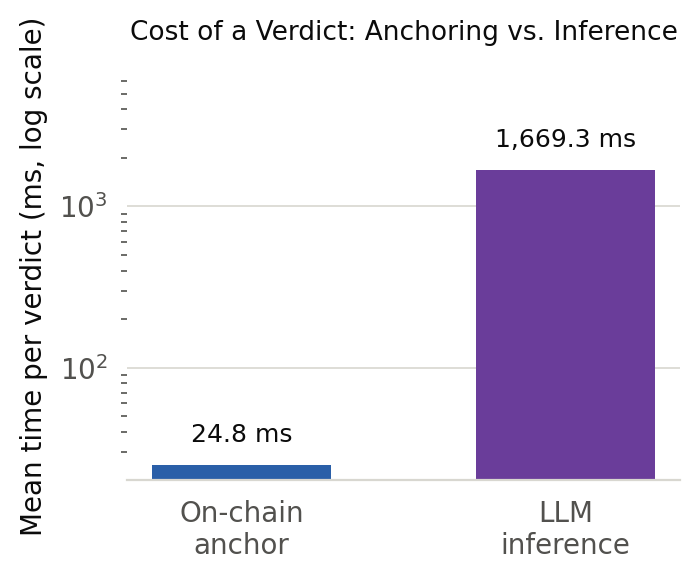
\includegraphics[width=\columnwidth]{figures/fig_latency.png}
\caption{Mean cost per verdict, on-chain anchoring versus LLM inference (log scale). Anchoring is the pipeline's cheap step; inference dominates cost by roughly three orders of magnitude.}
\label{fig:latency}
\end{figure}

\subsection{Verdict tamper-evidence}

Over \textbf{40} trials, mutating a stored verdict's severity score after anchoring was detected in \textbf{40} cases --- a \textbf{100\% detection rate} --- with \textbf{0 false positives} across the paired unmodified-record checks. This result is independent of Section 6.1--6.2's accuracy findings and should be read separately: it confirms that whatever the model decided --- right or wrong --- that decision, once anchored, cannot be silently altered by anyone, including an operator embarrassed by exactly the kind of misclassification Section 6.2 documents. We additionally confirmed directly that an anchored verdict's digest is recoverable from its mined transaction's raw input data, independent of anything the backend claims about the anchor having succeeded.

\begin{figure}[!t]
\centering
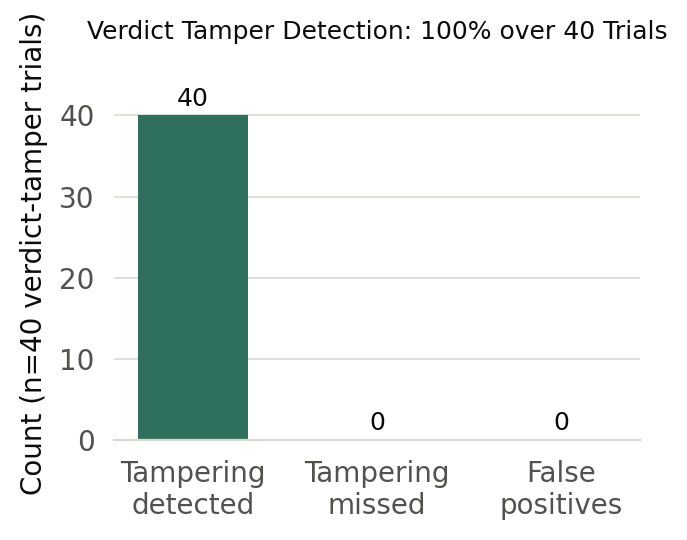
\includegraphics[width=\columnwidth]{figures/fig_tamper.png}
\caption{Verdict tamper-detection outcome. Every attempted post-hoc mutation of an anchored verdict's severity score was detected, with no false positives on the paired unmodified-record checks.}
\label{fig:tamper}
\end{figure}

\begin{table}[!t]
\centering
\caption{Summary of measured results against the live stack.}
\label{tab:results}
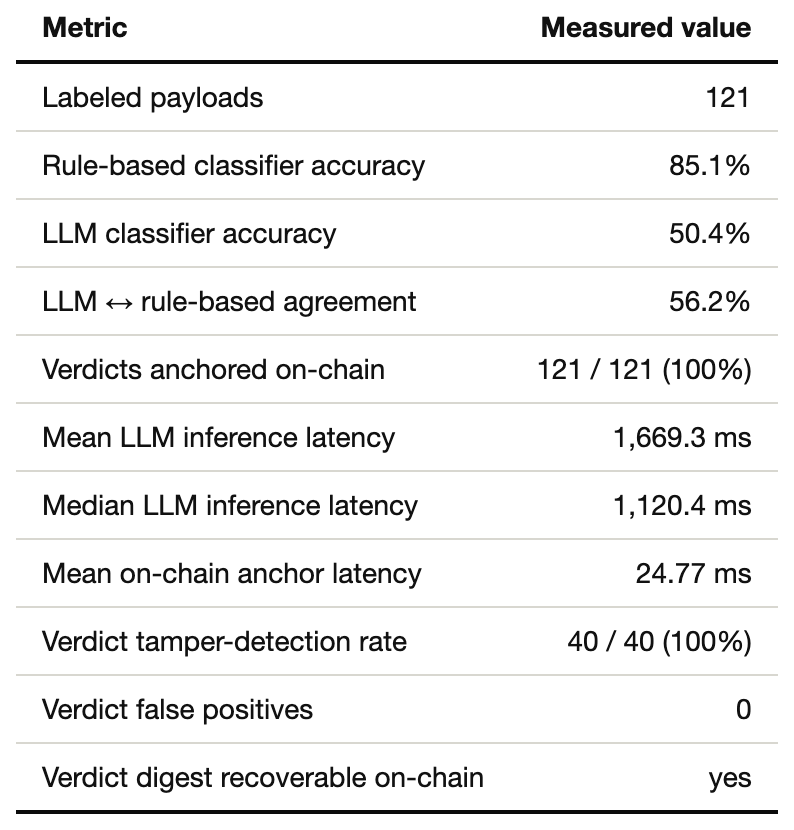
\includegraphics[width=\columnwidth]{figures/tab_results.png}
\end{table}

\begin{table*}[!t]
\centering
\caption{Per-category accuracy and the rule-based-minus-LLM accuracy gap, in percentage points, for every intent category in the labeled payload set.}
\label{tab:category}
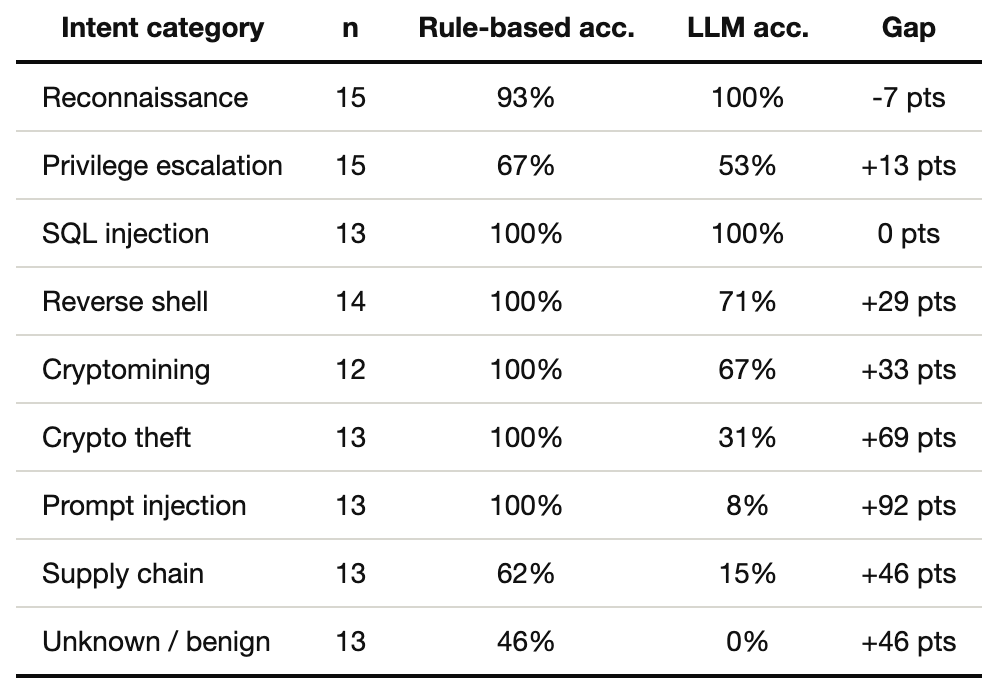
\includegraphics[width=\textwidth]{figures/tab_category.png}
\end{table*}

\section{Discussion}

\subsection{A close reading of the prompt-injection failures}

The prompt-injection category is the LLM classifier's single worst result (8\% accuracy), and it is worth reading closely because the failure mode is different from the generic "defaults to reconnaissance" pattern that explains most of the rest of Section 6.2. Several of the misclassified prompt-injection payloads in our set are framed as innocuous requests --- a role-play scenario, an appeal to authority ("this is a test environment"), a request framed as clarifying the system's own configuration --- and the model's own stated rationale for its (wrong) verdict on these payloads tends to engage with the payload's surface framing rather than recognizing the framing itself as the attack. This is consistent with, though not conclusive proof of, the injected instruction partially succeeding at reframing how the classifier characterizes its own input --- a small but concrete illustration of why using an LLM to classify adversarial text is a fundamentally harder problem than using it to classify text that is merely difficult, and a direct empirical instance of the concern raised in Section 2.3.

\subsection{What the anchoring layer does and does not fix}

It is tempting to read a tamper-evident verdict trail as a mitigation for the accuracy problem in Section 6.1--6.2. It is not, and treating it as one would be a mistake with real consequences. Anchoring guarantees that a verdict, once issued, cannot be silently changed --- it says nothing about whether the verdict was right. A 50.4\%-accurate classifier whose every output is perfectly tamper-evident is still a 50.4\%-accurate classifier: the anchoring layer's contribution is that the 34.7-point gap documented in this paper is now a fact that can be independently verified and cannot be quietly minimized after deployment, not a fact that the anchoring layer causes to shrink. This is precisely the accountability property motivated in Section 3: it does not make the AI better, it makes the AI's track record impossible to falsify, which is a precondition for anyone --- an operator, an auditor, a future version of this research --- being able to trust a reported accuracy number for this or any other deployed classifier in the first place.

\subsection{Deployment guidance given the measured gap}

Given results this lopsided, the deployment recommendation is not "replace the rule-based classifier with the LLM" --- the data does not support that --- nor is it "the LLM has no role," since it does add value on the categories where it matches or exceeds the rules (Section 6.2) and its free-text rationale is a form of triage context the rule-based classifier cannot produce at all. The recommendation the data supports is: treat the LLM verdict as a secondary, anchored second opinion alongside the primary rule-based signal, route disagreements (56.2\% of traffic in this benchmark) to a human reviewer rather than trusting either classifier's tie-breaking instinct, and treat any single-classifier deployment of the LLM alone on the categories where Section 6.2 shows it fails badly --- prompt injection and crypto theft above all --- as actively unsafe until the accuracy gap is closed by the improvements identified in Section 9.

To make this recommendation concrete, it is useful to walk through what each of three plausible deployment configurations would have looked like against this paper's own benchmark. A \textbf{rules-only} configuration --- the deployment's status quo before this paper's contribution --- achieves 85.1\% accuracy at effectively zero marginal latency and zero anchoring cost if the operator chooses not to anchor rule-based verdicts, but produces no free-text rationale and cannot improve without an engineer manually extending the rule list, which is precisely the coverage limitation Section 2.1 describes as the traditional motivation for introducing an LLM in the first place. An \textbf{LLM-only} configuration, replacing the rules outright, would have dropped the deployment's effective accuracy to 50.4\% --- a regression, not an improvement, and specifically a dangerous one on the crypto-theft and prompt-injection categories where the rule-based classifier was catching real attacks the LLM alone would have missed. A \textbf{routed-disagreement} configuration, as recommended above --- run both, act automatically only when they agree, and queue the 56.2\%-disagreement fraction for human review --- would have preserved the rule-based classifier's 85.1\% coverage on the categories it already handles well while surfacing the LLM's free-text rationale as additional context precisely on the harder cases a human reviewer benefits most from seeing, at the cost of routing a substantial fraction of traffic to a human queue rather than fully automating triage. Which of these three is the right choice for a given deployment depends on factors this paper's benchmark does not measure --- the volume of traffic a human reviewer can realistically absorb, the cost of a missed detection versus the cost of an analyst's time --- but the routed-disagreement configuration is the only one of the three that does not require accepting either the rule-based classifier's coverage ceiling or the LLM's measured error rate as a given, which is why it is the configuration we recommend as a starting point pending the accuracy improvements identified in Section 9.

\subsection{Generalization beyond this deployment}

Our results are measured against one model (Llama-3.1-8B-Instruct via OpenRouter), one fixed prompt, one honeypot's payload distribution, and 121 labeled examples; we do not claim these exact percentages generalize to a different model, a tuned prompt, or a different attack population. What we expect to generalize is the \emph{shape} of the finding: a fallback-to-generic-label failure mode under weak signal, disproportionate vulnerability on adversarially framed input, and --- most importantly for the paper's central argument --- the fact that any of these failure modes, in any deployment, are worth having a verifiable, unfalsifiable record of. That argument does not depend on which model was tested or how accurate it turned out to be; it depends only on the model being fallible, which every model is.

\subsection{The economics of anchoring an unreliable signal}

A natural objection to this paper's design is that anchoring is expensive relative to what it protects: why pay even 24.77 ms and a blockchain transaction to make tamper-evident a verdict that is wrong roughly half the time? The objection has real force and is worth answering directly rather than dismissing. The answer is that the anchoring cost is not proportional to the verdict's accuracy, and should not be evaluated as if it were --- a wrong verdict is not a cheaper event to falsify than a right one, and an operator's incentive to quietly alter a wrong verdict (Section 3.1's second adversary) is, if anything, stronger than their incentive to alter a correct one, precisely because the wrong verdict is the one that looks bad. Put differently: the case for anchoring gets \emph{stronger}, not weaker, as classifier accuracy falls, because a lower-accuracy classifier generates more embarrassing verdicts and therefore more instances of the exact incentive the anchoring layer is designed to remove. Section 6.4's finding that anchoring cost (24.77 ms) is three orders of magnitude smaller than classification cost (1,669.3 ms) also means the economic objection, even if one were sympathetic to it, targets the wrong component: eliminating anchoring saves a small fraction of the total cost a verdict already incurs from the LLM call it depends on.

\subsection{What an operator should watch for beyond aggregate accuracy}

Section 6.1's headline figures (85.1\% vs. 50.4\%) are a starting point for an operator evaluating whether to deploy an LLM classifier, but Section 6.2's per-category breakdown is the number that should actually drive the decision, because aggregate accuracy can look acceptable while concealing a category-specific failure with disproportionate real-world cost. A classifier at 50.4\% aggregate accuracy that fails almost completely on crypto theft and prompt injection --- as ours does --- is a materially worse deployment choice than a hypothetical classifier at the same aggregate accuracy whose errors are spread evenly across categories, because the former's blind spots align with the categories where a miss is most expensive (a drained wallet, a successfully manipulated model). We recommend that any operator evaluating an LLM classifier for a security-triage role compute and inspect the per-category breakdown before deployment, not only the aggregate number, and that any procurement or internal-approval process for such a system require the per-category table as a matter of course rather than accepting a single headline accuracy figure as sufficient evidence of readiness.

\subsection{Implications for model selection and benchmark design in security applications}

A broader implication of this paper's method, independent of its specific accuracy numbers, concerns how security teams should evaluate candidate LLM classifiers before adopting one. General-purpose LLM benchmarks --- reasoning tests, coding evaluations, broad knowledge quizzes --- are a poor proxy for the specific question a security team actually needs answered, which is not "how capable is this model in general" but "how does this model perform on the specific taxonomy of intents my system needs to distinguish, under my system's specific prompt, against my system's specific traffic distribution." A model that scores well on general benchmarks could, in principle, still exhibit the reconnaissance-default failure mode this paper documents (Section 6.2), because general benchmarks rarely test the specific behavior that failure mode depends on: how a model behaves when it lacks confident signal for a fine-grained categorical decision, under a fixed, unadorned prompt, on inputs specifically constructed to be difficult rather than typical. This is not a criticism of general-purpose benchmarks, which serve a different and legitimate purpose; it is an argument that they should not be treated as a substitute for the kind of task-specific, baseline-comparative evaluation this paper performs. A security team selecting among candidate models or prompt designs for a classification role should, at minimum, construct a labeled set representative of their own traffic --- following the ground-truth discipline described in Section 5.2 --- and measure per-category accuracy against their own existing baseline, rather than inferring likely production performance from a model's standing on unrelated public leaderboards. We offer this paper's methodology, more than its specific percentages, as a template for that evaluation: build the comparison against the system already in production, hold the prompt fixed and simple as a baseline before optimizing it, and report the full per-category breakdown rather than only the number that is most flattering to report.

\section{Limitations}

Our labeled set, at 121 payloads across nine categories, supports the aggregate and per-category comparisons in Section 6 but is not large enough to support fine-grained sub-category analysis (for instance, whether the LLM classifier fails differently on blind versus error-based SQL injection); a substantially larger and more diverse labeled corpus is needed before this paper's per-category percentages should be treated as precise population estimates rather than a directional finding. We evaluate exactly one LLM and one fixed, unoptimized prompt, by deliberate design (Section 3.4) --- the accuracy numbers in this paper are a baseline, not a ceiling, and Section 9 identifies the natural next experiments to establish how much of the gap is model choice, prompt design, or an inherent limit.

The tamper-detection experiment mutates a verdict's severity field specifically; while the canonicalization scheme in Section 4.2 gives no reason to expect a different mutated field to behave differently, we have not exhaustively tested every field, and a full taxonomy of verdict-tampering strategies analogous to the tampering taxonomies developed for raw-evidence anchoring (deletion of a verdict, truncation of a run of verdicts, consistent substitution of a verdict together with a re-derived digest) is future work rather than something this paper measures directly. Our threat model (Section 3.1) treats the classification pipeline's non-determinism as a fault we defend against structurally, but we have not run a dedicated stress test for it at scale; the zero-false-positive result in Section 6.5 is evidence within the scope of the trials run, not an exhaustive proof. The ground-truth labels themselves, while assigned independently of both classifiers under the behavioral discipline described in Section 5.2, were assigned by the same research team that built the system, which is a standard but real limitation of any single-team benchmark; an independently labeled or crowd-verified version of the payload set would strengthen the accuracy claims further. Finally, our benchmark measures the LLM classifier's behavior on payloads that were, ultimately, authored by the same team evaluating it, and while we drew on established, publicly documented attack patterns for each category rather than inventing artificial ones, we cannot rule out that a real attacker population would produce a payload distribution the model handles somewhat differently, in either direction, from what Section 6 reports.

A final limitation concerns the single-provider nature of our LLM access: all inference in this paper runs through one hosted API (OpenRouter) serving one model family, which means our measurements cannot separate the effect of the model's own weights from any provider-side behavior --- request routing, quantization, or serving-infrastructure choices a hosted API abstracts away from the caller and that a paper relying on that API cannot fully inspect or control. A locally hosted, fully specified model would close this gap at the cost of the operational simplicity a hosted API provides, and we regard that tradeoff as reasonable for a first measurement of the phenomenon this paper studies, while noting it as a boundary on precisely what "the model" refers to in our results.

\section{Future Work}

The most direct follow-up is closing the accuracy gap through the improvements this paper deliberately withheld to keep the baseline honest: few-shot prompting with examples drawn from the categories where Section 6.2 shows the largest gaps, a larger or differently trained model, and an explicit "abstain" option in the output schema to test whether allowing the model to decline a guess reduces the reconnaissance-default pattern documented in Section 6.2 --- since a model permitted to say "uncertain" may fail more gracefully than one forced into a confident wrong answer. A second direction is the ensemble design motivated in Section 7.3: formally defining and measuring a combined-classifier system that routes disagreements to review, rather than only observing the disagreement rate as this paper does, and quantifying how much of the rule-based classifier's advantage the ensemble can recover without losing the LLM's contribution on the categories (Section 6.2) where it already matches or exceeds the rules.

A third direction is extending the tamper-evidence evaluation to the full taxonomy of verdict-tampering strategies identified in the limitations above --- field-level edits beyond severity, wholesale deletion, and truncation of the verdict history --- with dedicated experiments for each, following the same discipline evidence-anchoring work applies to raw captured data (Section 2.5). A fourth, motivated directly by Section 7.1, is a dedicated adversarial-robustness evaluation isolating prompt-injection payloads specifically designed to manipulate the classifier's own verdict, to characterize how much of that category's poor performance is attributable to injected-instruction interference versus ordinary classification difficulty --- for instance, by comparing the model's behavior on prompt-injection payloads phrased as direct commands against semantically equivalent payloads phrased as indirect or socially engineered requests, to isolate whether framing specifically, rather than topic difficulty generally, drives the collapse in Table II.

A fifth direction follows from Section 2.6 and Section 7.5: a staged or confidence-gated architecture that runs the cheap rule-based classifier first and reserves the expensive LLM call for payloads the rule-based classifier flags as ambiguous or unmatched, which would test whether restricting the LLM's workload to genuinely hard cases changes its accuracy profile relative to the unconditional deployment this paper measures --- plausibly for the better, if the categories where the rule-based classifier already performs well are exactly the categories where the LLM's marginal contribution is smallest. A sixth and more ambitious direction is a longitudinal field deployment: running the dual-classification pipeline against a public-facing honeypot for an extended period, collecting a much larger and organically-arriving payload set than any hand-constructed benchmark can provide, and re-measuring the accuracy gap and confusion pattern against real, uncurated attacker traffic rather than the authored payload set this paper uses.

\section{Reproducibility}

Every number in this paper is generated, not hand-entered, and the mechanism by which that holds is worth stating precisely, both because it is a methodological commitment consistent with the paper's own argument about auditability and because it lets a reader reproduce or challenge any figure directly rather than taking it on trust.

\textbf{System prompt.} The LLM classifier is instructed with a single fixed system prompt naming the nine permissible intent categories exactly, requesting a severity score on a 0--100 integer scale, requesting a rationale capped at twelve words, and specifying the output format as one line of compact JSON with no surrounding commentary or markdown formatting --- the same prompt is used for every payload in every category, with no per-category or per-service variation, so that Section 6.2's per-category accuracy differences reflect the model's own differential difficulty with each category rather than differences in how the categories were prompted for.

\textbf{Model and provider.} All LLM calls in this paper's benchmark run against \texttt{meta-llama/llama-3.1-8b-instruct} served via OpenRouter, at temperature 0 and an 80-token output cap, chosen to keep responses short, deterministic, and inexpensive to call at the volume the benchmark requires; a higher-temperature or larger-context configuration was not evaluated and is not implied to perform identically.

\textbf{Ledger.} All anchoring in this paper runs against a local Ganache development chain (chain ID 1337), which mines transactions effectively instantly; Section 7 and the discussion of anchoring cost (Section 6.4) should be read with this in mind, in the same way the companion evidence-anchoring literature (Section 2.5) is explicit about the same development-chain caveat.

\textbf{Build pipeline.} The benchmark harness submits every labeled payload to the live backend, records the LLM's verdict, the rule-based classifier's verdict, and the timing of each pipeline stage into a single machine-readable results file, and every figure, table, and inline statistic in this paper --- including the abstract's headline numbers --- is substituted into the paper text directly from that file by an automated build step. Re-running the benchmark against the live stack and rebuilding the paper regenerates every number, chart, and table consistently; there is no manual editing step between the measurement and the published figure that could introduce drift between what was measured and what is reported. Because the LLM calls are live network requests to a hosted model, re-running the benchmark is expected to reproduce the qualitative pattern of results (rule-based classifier outperforming the LLM classifier, errors concentrated in the same categories) rather than reproducing the exact percentages in this paper bit-for-bit, since model providers can update served weights and hosted inference carries ordinary network and load variance; this expectation is itself consistent with Section 7.4's claim that the \emph{shape} of the finding, not the exact numbers, is what should be expected to generalize.

\section{Conclusion}

We built an LLM-driven intent classifier into a live honeypot, ran it head-to-head against the deployment's existing rule-based classifier on 121 identical, hand-labeled payloads, and anchored every verdict --- right or wrong --- on an Ethereum-compatible ledger so that what the model concluded cannot be silently altered after the fact. The honest result is that the LLM classifier, evaluated as a straightforward, unoptimized baseline, is substantially less accurate than the rules it was meant to complement (50.4\% versus 85.1\%), with failures concentrated in exactly the categories --- prompt injection, crypto theft, and benign traffic --- where a wrong answer costs the most. The anchoring layer does not fix this gap and was never intended to; measured separately, it adds a modest 24.77 ms per verdict, anchors successfully 100\% of the time, and detected 100\% of attempted post-hoc tampering with 0 false positives.

Together, these results support a narrower and more defensible claim than "AI improves honeypot triage": an AI classifier deployed in a security-decision role is a fallible witness, its failure modes are measurable and non-uniform, and its verdicts belong in a tamper-evident record for the same reason any fallible witness's testimony does --- not because the record makes the testimony true, but because it makes the testimony impossible to quietly rewrite once its flaws become apparent. The two contributions of this paper are, deliberately, not separable: a measurement of an AI system's failure modes is only as trustworthy as the record of that measurement is tamper-evident, and a tamper-evident record of an AI system's decisions is only as valuable as the accuracy of what it records has been honestly established. Neither half, published alone, would have supported the claim the two halves support together.

More broadly, we read this paper's result as a caution against a specific, common pattern in applied AI deployment: introducing a general-purpose model into a role a narrower, purpose-built system previously filled, on the strength of the general-purpose model's broad capability, without first measuring whether that capability actually transfers to the specific task at hand under the specific conditions of the deployment. The rule-based classifier this paper benchmarks against is, by any reasonable standard, a primitive piece of software --- a fixed list of keyword and pattern rules an experienced engineer could read in an afternoon. That primitive system outperforming a modern large language model on the majority of this paper's nine categories is not an indictment of large language models in general; it is a demonstration that generality and task-specific reliability are different properties, that a system's fluency is not evidence of its accuracy, and that the only way to know which property a given deployment actually needs --- and whether the system in front of you has it --- is to measure directly, on the actual task, against the actual alternative, and to keep an honest, unfalsifiable record of what that measurement found.

\section{Acknowledgment}

The authors thank the Department of Computer Science and Engineering at Amrita School of Computing, Coimbatore, for the infrastructure and guidance supporting this work, and acknowledge OpenRouter and the maintainers of the underlying Llama model family for the hosted inference access this evaluation depends on, and the maintainers of Ganache and the supporting Ethereum client libraries used for the anchoring benchmark described in Section 5.

% ==== References ====

\begin{thebibliography}{00}
\bibitem{ref1} L. Spitzner, Honeypots: Tracking Hackers. Boston, MA, USA: Addison-Wesley, 2003.
\bibitem{ref2} N. Provos and T. Holz, Virtual Honeypots: From Botnet Tracking to Intrusion Detection. Upper Saddle River, NJ, USA: Addison-Wesley, 2007.
\bibitem{ref3} S. Nakamoto, "Bitcoin: A peer-to-peer electronic cash system," 2008. [Online]. Available: \url{https://bitcoin.org/bitcoin.pdf}
\bibitem{ref4} G. Wood, "Ethereum: A secure decentralised generalised transaction ledger," Ethereum Project Yellow Paper, 2014.
\bibitem{ref5} National Institute of Standards and Technology, "Secure Hash Standard (SHS)," FIPS PUB 180-4, 2015.
\bibitem{ref6} Truffle Suite, "Ganache: One-click blockchain --- a personal Ethereum blockchain for development," ConsenSys. [Online]. Available: \url{https://trufflesuite.com/ganache/}
\bibitem{ref7} B. Schneier and J. Kelsey, "Secure audit logs to support computer forensics," ACM Trans. Information and System Security, vol. 2, no. 2, pp. 159--176, 1999.
\bibitem{ref8} S. Bonomi, M. Casini, and C. Ciccotelli, "B-CoC: A blockchain-based chain of custody for evidences management in digital forensics," 2018. [Online]. Available: \url{https://arxiv.org/abs/1807.10359}
\bibitem{ref9} F. Perez and I. Ribeiro, "Ignore this title and HackAPrompt: Exposing systemic vulnerabilities of LLMs through a global prompt hacking competition," in Proc. EMNLP, 2023.
\bibitem{ref10} K. Greshake et al., "Not what you've signed up for: Compromising real-world LLM-integrated applications with indirect prompt injection," in Proc. ACM Workshop on Artificial Intelligence and Security (AISec), 2023.
\bibitem{ref11} S. Lin, J. Hilton, and O. Evans, "TruthfulQA: Measuring how models mimic human falsehoods," in Proc. ACL, 2022.
\bibitem{ref12} A. Xiong et al., "Can LLMs express their uncertainty? An empirical evaluation of confidence elicitation in LLMs," in Proc. ICLR, 2024.
\bibitem{ref13} R. Binns, "Fairness in machine learning: Lessons from political philosophy," in Proc. Conf. Fairness, Accountability, and Transparency (FAT-star), 2018, pp. 149--159.
\bibitem{ref14} M. Raji et al., "Closing the AI accountability gap: Defining an end-to-end framework for internal algorithmic auditing," in Proc. Conf. Fairness, Accountability, and Transparency (FAccT), 2020, pp. 33--44.
\bibitem{ref15} A. Ahmad, M. Saad, M. Al Ghamdi, D. Nyang, and A. Mohaisen, "BlockTrail: A service for secure and transparent blockchain-driven audit trails," IEEE Systems Journal, vol. 16, no. 1, pp. 1367--1378, 2022.
\bibitem{ref16} "LogStamping: A blockchain-based log auditing approach for large-scale systems," 2025. [Online]. Available: \url{https://arxiv.org/abs/2505.17236}
\end{thebibliography}

\vfill
\noindent\rule{0.48\textwidth}{0.4pt}\par
{\footnotesize This work is licensed under a Creative Commons Attribution
4.0 License. For more information, see
\url{https://creativecommons.org/licenses/by/4.0/}}

\end{document}
